%% \chapter[htoc-titlei][hhead-titlei]{htitlei}
%% -----------------------------------------------------------------------------
\chapter[Monte Carlo simulation][Monte Carlo simulation]{Monte Carlo simulation}
\label{ch:mc}

Monte Carlo (MC) simulations are an important tool for particle physics
experiments.
MC techniques are used to simulate physics processes that occur during
particle collisions.
These simulated events also include the interactions of the decay products
in the detector, and can be used to tune the selection of an analysis,
estimate the expected event yields and kinematic shapes, and ultimately,
evaluate the expected sensitivity of a particular search.
MC simulation of background and signal processes are used on ATLAS.
This chapter introduces some of the basic concepts of event generation, but
focuses on the generation of the $B-L$ stop pairs from the model described in
Section~\ref{sec:theory_bl_extension}.

MC simulation of particle physics events can be broken into two major parts.
The first step is the event generation, described in
Section~\ref{sec:event_gen}.
In the event generation stage, the actual Physics processes that occur as a
result of the collision are simulated.
This includes the hard interaction as well as the resulting decay of any
unstable particles.
As in the real detector, once the proton collisions are simulated, the decay
products travel through the detector, and may leave a measurable signature
which can be measured.
This involved material interactions with the detector, and is discussed in
Section~\ref{sec:det_sim}.

%% -----------------------------------------------------------------------------
\FloatBarrier
\section{Event Generation}
\label{sec:event_gen}

Before discussing the details of event generation, it is useful to first
introduce the concept of an ``event.''
At the LHC, beams of protons are accelerated in opposite directions, and
allowed to cross at specific locations as described in Section~\ref{sec:lhc}.
At each of these crossings, protons from the two beams collide with one
another, resulting in a spray of particles in the detector.
Each of these crossings represents a single event.
Figure~\ref{fig:mc_event} shows a pictorial representation of a simulated
$t\bar{t}H$ event.

\begin{figure}[p]
  \centering
  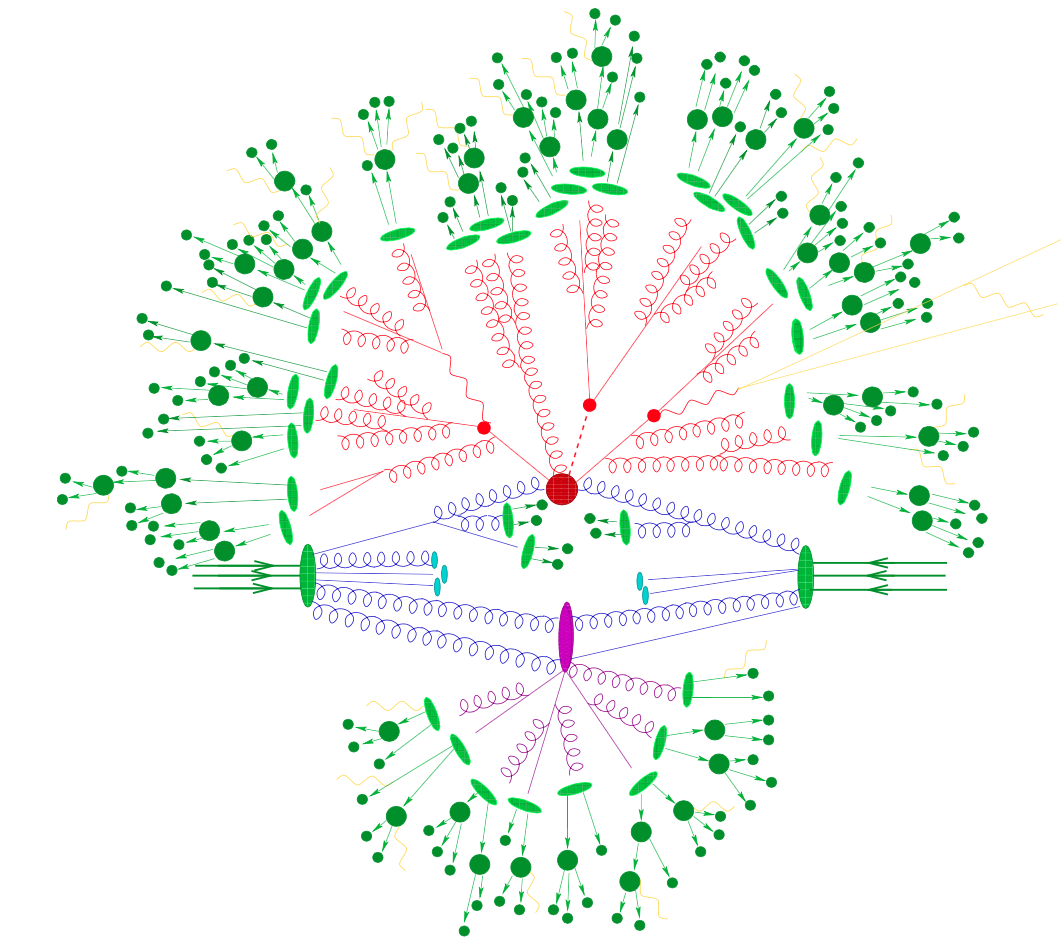
\includegraphics[width=\textwidth, clip=true, trim=0 0 0 0]
  {figs/mc_gen/full_mc_event.png}
  \caption[
    Pictorial representation of a $t\bar{t}H$ event as produced by an event
    generator~\cite{Gleisberg:2008ta}.
  ]{
    Pictorial representation of a $t\bar{t}H$ event as produced by an event
    generator.
    The hard interaction (big red blob) is followed by the decay of both top
    quarks and the Higgs boson (small red blobs).
    Additional hard QCD radiation is produced (red) and a secondary
    interaction takes place (purple blob) before the final-state partons
    hadronize (light green blobs) and hadrons decay (dark green blobs).
    Photon radiation occurs at any stage (yellow)~\cite{Gleisberg:2008ta}.
  }
  \label{fig:mc_event}
\end{figure}

Looking more closely at the interactions taking place, one notices that,
rather than the full protons interacting with each other, the interactions
take place between the constituent quarks and gluons within the two protons.
In some cases, there is a ``hard interaction,'' or an inelastic scattering
where additional particles are created.
This is mathematically represented by the ``matrix element'' calculation.
As the protons pass through each other, there are also soft interactions
between the constituent partons in a process called the ``underlying event.''
The underlying event produces charged particles and jets in the detector, in
addition to those coming from the hard interaction.

%% - - - - - - - - - - - - - - - - - - - - - - - - - - - - - - - - - - - - - - -
\FloatBarrier
\subsection{Underlying event}

%% - - - - - - - - - - - - - - - - - - - - - - - - - - - - - - - - - - - - - - -
\FloatBarrier
\subsection{Matrix element}

%% - - - - - - - - - - - - - - - - - - - - - - - - - - - - - - - - - - - - - - -
\FloatBarrier
\subsection{Parton shower}

%% - - - - - - - - - - - - - - - - - - - - - - - - - - - - - - - - - - - - - - -
\FloatBarrier
\subsection{Jet matching}
\label{sec:jet_matching}

{\color{red} Talk about matching. Probably use several figures to help explain
  this topic. Probably also talk about these DJR plots, and how we want them
  to look}

{\color{red} Add info about HFOR here}

%% -----------------------------------------------------------------------------
\FloatBarrier
\section{Detector simulation}
\label{sec:det_sim}

{\color{red} Probably something brief about how detector simulation is done, and
  the difference between full/fast sim}

